
\section{Method}\label{Sec:Method}

Based on the extensive literature review presented above, two different forecasting techniques were chosen to be employed to predict households' energy consumption and production. The following criteria were considered for the selection of appropriate methods: 

\begin{enumerate}
    \item The forecasting technique had to produce deterministic (i.e., point) forecasts.
    \item The forecasting technique had to be used in existing studies about forecasting energy consumption or production.
    \item The existing study or studies using the forecasting technique had to use comparable data, i.e., recorded by smart meters, 60-min resolution or less, recorded in multiple households, and not recorded in SMEs or other business or public buildings.
    \item The forecasting task had to be comparable to the forecasting task of this study, i.e., single consumer household in contrast to the prediction of aggregated energy time series and very short forecasting horizon ($\leq 24$ hours).
    \item The forecasting technique had to only take historical and calender features as input for the prediction.
    \item The forecasting technique had to produce absolutely and relative to other studies promisingly accurate predictions.
\end{enumerate}

% (1) The forecasting technique had to produce deterministic (point) forecasts. (2) The forecasting technique had to be used in existing studies about forecasting energy consumption or production. (3) The existing study or studies using the forecasting technique had to use comparable data. (4) The forecasting task had to be comparable to the forecasting task of this study, i.e., single consumer household and very short-term forecasting horizon. (5) The forecasting technique only employed historical and calender features as input for the prediction. (6) The forecasting technique had to produce absolute and relative to other studies promisingly accurate predictions.

\noindent Based on these criteria the following forecasting techniques were selected for the prediction task at hand: Pooling-based deep recurrent neural network (PDRNN) based on the procedure outlined by \citet{Shi:2017} and sparse autoregressive LASSO as developed and implemented by \citet{Li:2017}.%, and Kernel-Wavelet-Functional method (KWF) following the idea of \citet{Auder:2018} of using discrete wavelet transform and clustering before applying the KWF method.

% As the data used to train the models is in 3-minute intervals, but the prediction will have to be made 15 minutes ahead, all forecasting models will be used to make 5 sequential one-step ahead predictions. These 5 predictions will then be aggregated into a single forecast for the whole 15-minute interval and compared to the actual consumption/production within this 15-minute interval (i.e., the aggregation of the 5 corresponding 3-minute consumption values).



%%%%%%%%%%%%%%%%%%%%%%%%%%%
%%%   Benchmark model   %%%
%%%%%%%%%%%%%%%%%%%%%%%%%%%

\subsection{Benchmark model} \label{Sec:Method;Subsec:Benchmark}

Benchmark models serve as a trivial baseline to assess the relative improvement of a sophisticated model \citep{Meer:2018}. According to \citet{Pinson:2012}, a benchmark model should serve as a reference, need few computational resources to be estimated, and be model-free. A sophisticated forecasting method is only worth implementing if it can significantly outperform a trivial benchmark model \citep{Diagne:2013}. A frequent benchmark model used for deterministic forecasts is the simple persistence model \citep{Meer:2018}. This model assumes that the conditions at time $t$ persist at least up to the period of forecasting interest at time $t+h$. In energy forecasting, this na\"ive model is surprisingly well suited to forecast very short time periods of a few seconds or minutes \citep{Pinson:2012} and, thus, often harder to beat than it might seem. The persistence model is defined as
%
\begin{equation} \label{Eq:naivepred}
\widehat{x}_{t+1}=x_t.
\end{equation}

There are several other benchmark models commonly used in energy load forecasting. Most of them are, in contrast to the persistence model, more sophisticated benchmarks, such as the Holt-Winters-Taylor (HTW) exponential smoothing method \citep[see, e.g.,][]{Arora:2016}. Further sophisticated benchmark models are the Vanilla benchmark \citep{hong:2010}, and the popular ARMA method \citep{Box:1990}. However, as the forecasting task at hand serves the specific use case of being an input for the bidding process in a blockchain-based local energy market, the improvement of the forecasting model over a benchmark model is of secondary importance. The task here is not so much to establish the quality of a forecasting model per se as to assess whether the available and most promising forecasting techniques can deliver accurate enough results for the use case explained above. Hence, only the persistence model will serve as a benchmark to the forecasting techniques presented next. The more relevant test of the forecasting models' accuracy will be explained in Section \ref{Sec:Method;Subsec:Market}.



%%%%%%%%%%%%%%%%
%%%   LSTM   %%%
%%%%%%%%%%%%%%%%

\subsection{Long short-term memory recurrent neural network} \label{Sec:Method;Subsec:LSTM}

Even though being applied very successfully in a wide range of tasks, such as speech recognition \citep{Graves:2013} or anomaly detection in time series \citep{Malhotra:2015}, long short-term memory (LSTM) neural networks (NN) have been introduced only very recently in load forecasting studies \citep[e.g.,][]{Kong:2018,Shi:2017,Gan:2017,Chen:2018}. Compared to previous previous attempts using machine learning techniques, the application of LSTM neural networks for load forecasting has been much more successful \citep{Kong:2018,Shi:2017} as these studies benefit from the high effectiveness of recurrent neural networks for sequence learning. LSTM units are particularly well suited to learn long sequences or time series due to their ability to retain information over many time steps. The next three sections are based on \citet{chollet:2018}, \citet{Lipton:2015}, and \citet{Gan:2017}.



%%%%%%%%%%%
\subsubsection{Basic functioning of neural networks}

To understand the full advantage that LSTM recurrent neural networks have over other machine learning techniques for time series learning, it is useful to take a step back and recapitulate the basic functioning of a so-called feedforward neural network first. The most basic building blocks of any neural network are three types of layers: an input layer, one or more hidden layer(s), and an output layer. Each layer consists of one or more units (sometimes called neurons). Each unit in a layer takes in an input, applies a transformation to this input, and outputs it to the next layer (see Figure \ref{Fig:simpleNN}. Formally, this can be written as
%
\begin{equation} \label{feedforward}
\begin{split}
    \vec{h}_{1i}&=\phi_1\left(\vec{W}_1\vec{x}_i+\vec{b}_1\right)\\
    \vec{h}_{2i}&=\phi_1\left(\vec{W}_2\vec{h}_{1i}+\vec{b}_2\right)\\
    &\setbox0\hbox{=}\mathrel{\makebox[\wd0]{\hfil\vdots\hfil}}\\
    o_i&=\phi_n\left(\vec{W}_n\vec{h}_{(n-1)i}+\vec{b}_n\right)=\widehat{y}_i,
\end{split}
\end{equation}
%
where $n$ denotes a layer, $\phi_n$ is the activation function, $\vec{W}_n$ is the weight matrix, and $\vec{b}_n$ the bias vector in layer $n$. $\vec{x}_i$ is the $i^{th}$ input vector and $o_i$ the output of the output layer which is the estimation of the true value $y_i$.
%
\begin{figure}
    \centering
    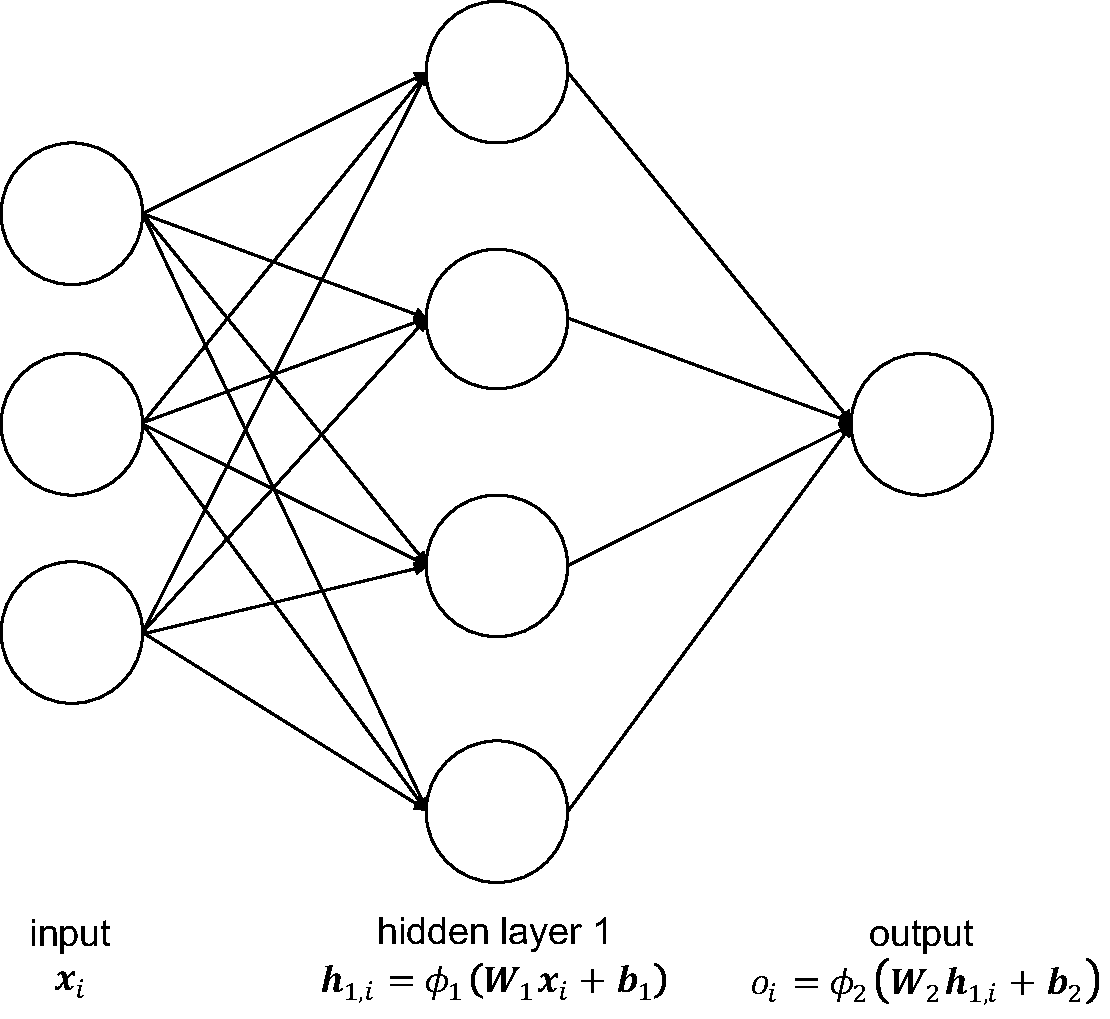
\includegraphics[scale=0.6]{thesis/figures/simpleNN.pdf}
    \caption[Schematic visualization of a simple neural network]{Schematic visualization of a simple neural network. Adapted from \citet{Gan:2017}.}
    \label{Fig:simpleNN}
\end{figure}

In the input layer there are as many units as there are features (i.e., variables) that serve as input for the forecasting model. The units of the input layer are connected to all units in the (first) hidden layer. The weight matrices and bias vectors in each layer are parameters that are adjusted during the training of the model. In all subsequent hidden layers, all units of one layer are connected to all units of the next layer (this is called densely connected). The last layer consists of as many units as there are output values. That is, if the forecasting model should just predict a single value, the output layer will have a single unit that takes in the weighted output values of all units of the last hidden layer, applies a transformation to these inputs and outputs a single value. The transformation that is applied to the input within each unit is called activation function and must be chosen depending on the task at hand. Especially for sequence learning, this activation function is often a hypberbolic tangent (tanh) \citep{Lipton:2015}:

\begin{equation} \label{activation}
    \phi(z)=\frac{e^z-e^{-z}}{e^z+e^{-z}}
\end{equation}

The learning in machine learning refers in the case of neural networks to adjusting the weight matrices and bias vectors such that the best prediction is output. In supervised learning, adjusting these weights (i.e., the training of the model) is done through an algorithm that is called backpropagation which was introduced by \citet{Rumelhart:1986}. First, the weight matrices and bias vectors are randomly initialized. Then, in a first iteration, the training data is fed into the network, which outputs a prediction. This prediction is assessed with the help of a loss function that quantifies the distance between the prediction and the true value. A commonly used loss function is the mean absolute error:
%
\begin{equation} \label{lossMAE}
    L\left(y, \widehat{y}\right)=\text{MAE}=\frac{1}{N}\sum_{i=1}^N\left|\widehat{y}_i-y_i\right|
\end{equation}
%
The simplest method to optimize the model parameters is to compute the derivative of the loss function with respect to each parameter in the model and change each parameters in a fixed-size step in the direction of the negative gradient. This method is called gradient descent. Thereby the prediction error is "backpropagated" through the network to update the parameters. This is repeated in each iteration until the model converges to a value of the loss function that cannot be further improved.



%%%%%%%%%%%
\subsubsection{Recurrent neural networks}

The problem for time series learning with feedforward neural networks is that they do not have an internal state that could retain a memory. That is, to learn a sequence or time series, a feedforward neural network would always need the complete time series as a single input as it cannot retain the state learned in a previous chunk of the time series to apply it to the next chunk fed into the model. This problem is solved by recurrent neural networks.

Recurrent neural networks still consist of the basic building blocks of units and layers. However, the units do not just feed forward the transformed input as output but have a recurrent connection that feeds an internal state back into the unit as input (see Figure \ref{Fig:RNNunit}. Thereby, a RNN unit loops over individual elements of an input sequence, instead of processing the whole sequence in a single step. This means, the RNN unit applies the transformation to the first element of the input sequence and combines it with its internal state. This introduces the notion of time into neural networks. Formally, this can be written as
%
\begin{equation} \label{RNN}
\begin{split}
    \vec{h}_{1,t}&=\phi_1\left(\vec{W}_1^{(i)}\vec{x}_t+\vec{W}^{(r)}_1\vec{h}_{1,(t-1)}+\vec{b}_1\right)\\
    \vec{h}_{2,t}&=\phi_2\left(\vec{W}_2^{(i)}\vec{h}_{1,t}+\vec{W}^{(r)}_2\vec{h}_{2,(t-1)}+\vec{b}_2\right)\\
    &\setbox0\hbox{=}\mathrel{\makebox[\wd0]{\hfil\vdots\hfil}}\\
    o_t&=\phi_n\left(\vec{W}_n^{(i)}\vec{h}_{(n-1),t}+\vec{b}_n\right)=\widehat{y}_t,
\end{split}
\end{equation}
%
where $n$ denotes a layer, $\phi_n$ is the activation function, $\vec{W}_n^{(i)}$ is the weight matrix for the input, $\vec{W}_n^{(r)}$ is the weight matrix for the recurrent input (i.e., the output of layer $n$ in the previous time step), and $\vec{b}_n$ the bias vector in layer $n$. $\vec{x}_i$ is the $i^{th}$ input vector and $o_i$ the output of the output layer which is the estimation of the true value $y_i$. Note that the output layer has no recurrent units but is the same as in a simple feed forward network.
%
\begin{figure}
    \centering
    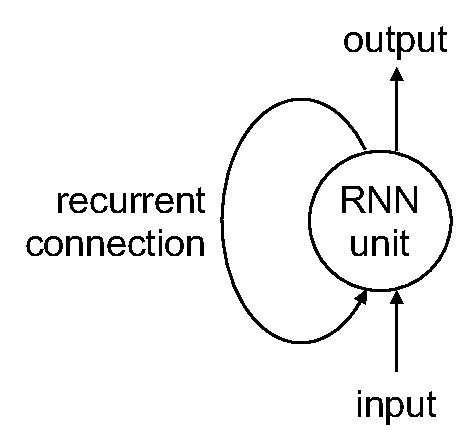
\includegraphics[scale=0.6]{thesis/figures/RNNunit.pdf}
    \caption[Schematic visualization of a RNN unit]{Schematic visualization of a RNN unit. Adapted from \citet{chollet:2018}.}
    \label{Fig:RNNunit}
\end{figure}
%
The cyclical structure of RNN can be unrolled across time (see Figure \ref{Fig:RNNunfolded}). This illustrates that a RNN is still trainable through backpropagation across all time steps. This is called backpropagation through time (BPTT) and was introduced by \citet{Werbos:1990}. Theoretically, this structure enables RNN to retain information about sequence elements that have been processed many steps before the current step and use it for the prediction of the current step. However, in practice the vanishing gradient problem occurs\footnote{For more details on the vanishing gradient problem see, e.g., \citet{Bengio:1994}}. This problem makes RNNs for very long sequences basically untrainable.
%
\begin{figure}
    \centering
    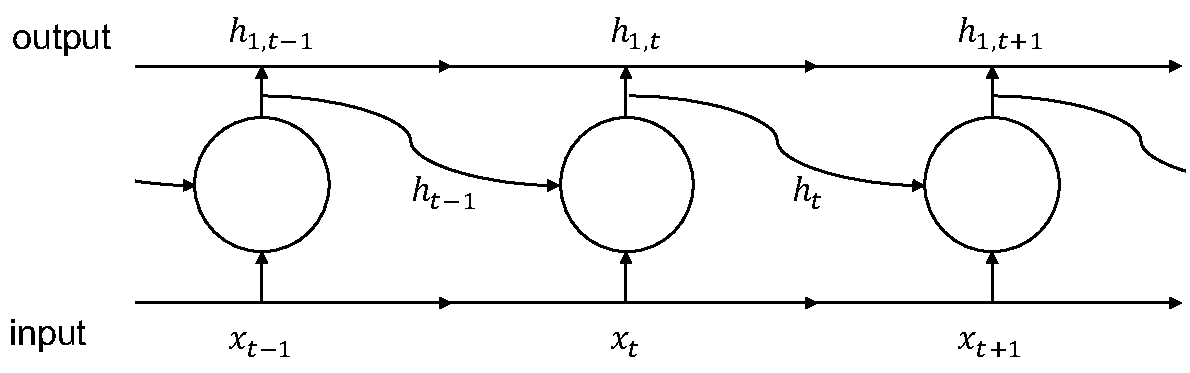
\includegraphics[scale=0.6]{thesis/figures/RNNunfolded.pdf}
    \caption[Schematic visualization of an unfolded RNN unit]{Schematic visualization of an unfolded RNN unit. Adapted from \citet{chollet:2018}.}
    \label{Fig:RNNunfolded}
\end{figure}



%%%%%%%%%%%
\subsubsection{RNN with long short-term memory units}

To overcome the vanishing gradient problem, \citet{Hochreiter:1997} developed LSTM units. LSTM units extend RNN units by an additional state. This state can retain information for as long as needed. In which step this additional state is updated and in which state the information it retains is used in the transformation of the input is controlled by three so-called gates\footnote{In their original specification, \citet{Hochreiter:1997} included only two gates. However, as this LSTM specification was still prone to the vanishing gradient problem under some circumstances, \citet{Gers:2000} extended it by a third gate.}. These three gates again have the form of a simple RNN cell. Formally, these gates can be written as (following the notation of \citet{Lipton:2015})
%
\begin{equation} \label{LSTMgates}
\begin{split}
    \vec{i_t}&=\sigma\left(\vec{W}^{(ix)}\vec{x}_t+\vec{W}^{(ih)}h_{t-1}+\vec{b_i}\right)\\
    \vec{f_t}&=\sigma\left(\vec{W}^{(fx)}\vec{x}_t+\vec{W}^{(fh)}h_{t-1}+\vec{b_f}\right)\\
    \vec{o_t}&=\sigma\left(\vec{W}^{(ox)}\vec{x}_t+\vec{W}^{(oh)}h_{t-1}+\vec{b_o}\right),
\end{split}   
\end{equation}
%
where $\sigma$ is the sigmoid activation function $\sigma(z)=\frac{1}{1+e^{-z}}$, with $W$ denoting the weight matrices that are intuitively labeled ($ix$ for the weight matrix of gate $i_t$ multiplied with the input $x_t$ etc.), and $b$ denoting the bias vectors.\footnote{Sometimes, the gates are titled input, output, and forget gate. However, as \citet{chollet:2018} put it:
\begin{quote}
    "[T]hese interpretations don’t mean much, because what these [gates] actually do is determined by the contents of the weights parametrizing them; and the weights are learned in an end-to-end fashion, starting over with each training round, making it impossible to credit this or that operation with a specific purpose." (p. XX)
\end{quote}
}

Again following the notation of \citet{Lipton:2015}, the full algorithm of a LSTM unit is given by the three gates specified above, the input node
%
\begin{equation} \label{LSTMinput}
    \vec{g_t}=\sigma\left(\vec{W}^{(gx)}\vec{x}_t+\vec{W}^{(gh)}h_{t-1}+\vec{b_g}\right),
\end{equation}
%
the internal state of the LSTM unit at time step $t$
%
\begin{equation} \label{LSTMstate}
    \vec{s}_t=\vec{g}_t\odot\vec{i}_t+\vec{s}_{t-1}\odot\vec{f}_t,
\end{equation}
%
where $\odot$ is pointwise multiplication, and the output at time step $t$
%
\begin{equation} \label{LSTMoutput}
    \vec{h}_t=\phi\left(\vec{s}_t\right)\odot\vec{o}_t.
\end{equation}
%

To summarize, all neural networks use the basic building blocks of units that form input, hidden, and output layers. The training process of neural networks involves updating the parameters (weights and biases) of the model based on the gradient descent of a loss function that quantifies the accuracy of a prediction compared to true values. RNN enables the neural network to process individual elements of a sequence or time series sequentially and still use information that was obtained in previous time steps for the current transformation of the input. LSTM RNN is an extension of simple RNN which has the advantage of being able to retain a state over multiple time steps and solves the vanishing gradient problem through the introduction of an additional internal state $\vec{s}_t$. By this, LSTM RNN are capable of learning highly complex, non-linear relationships in time series data which makes it a promising forecasting technique to predict households' very short-term energy consumption and production.



%%%%%%%%%%%
\subsubsection{Model training}



%%%%%%%%%%%%%%%%%
%%%   LASSO   %%%
%%%%%%%%%%%%%%%%%

\subsection{Sparse auto-regressive LASSO} \label{Sec:Method;Subsec:LASSO}



%%%%%%%%%%%%%%%%%%%%%%%%%%
%%%   Error measures   %%%
%%%%%%%%%%%%%%%%%%%%%%%%%%

\subsection{Error measures} \label{Sec:Method;Subsec:Error}

Error measures play an essential role in any prediction task. Also called performance metrics, these measures are used to quantify the accuracy of the prediction generated by a forecasting model \citep{zor:2017}. Without assessing the prediction accuracy through error measures, it is impossible to quantify whether the proposed forecasting technique is an improvement compared to the benchmark models \citep{Meer:2018}. Moreover, error measures are used by supervised machine learning algorithms to assess the prediction accuracy in cross-validation and to accordingly adjust their parameters.

However, there is a wide variaty of error measures available and actively used in the research of energy forecasting. \citet{zor:2017} reviewed the energy forecasting literature published in 2017 and found eight different error measures that were used to assess the forecasting accuracy. Among those, mean absolute percentage error was used in 83 \% of the studies, with mean absolute error and root mean squared error coming third and second with 32 and 31 \% respectively. As these results suggest, there is a lack of standardization in the field of energy forecasting regarding the usage of the various available error measures \citep{Meer:2018}. This is aggravated by the fact, that different error measures are appropriate in different use cases and cannot be generally applied without careful consideration. Therefore, the following section introduces the error measures used in the research at hand and discusses their advantages and disadvantages. Following the suggestion of \citet{Hoff:2013} several performance metrics will be used to evaluate the quality of the forecast models. The choice of performance metrics is mostly guided by the compilation provided by \citet{Meer:2018}.


%%%%%%%%%%%
\subsubsection{MAE and RMSE}

Error measures can be classified into representing absolute or percentage errors \citep{Hoff:2013}. Absolute error measures are, for example, mean absolute error (MAE) and root mean squared error (RMSE). Both are quite popular as performance metrics for energy forecasts \citep{zor:2017}. Absolute error measures can be formulated in terms of a vector function 
%
\begin{equation} \label{Eq:vectorfunction}
    E=F\left(\vec{f}, \vec{x}\right),
\end{equation}

\noindent where $\vec{f}$ and $\vec{x}$ are the forecasted and actual data vectors respectively \citep{Haben:2014}. The metric $F$ is then the absolute p-norm,
%
\begin{equation} \label{Eq:pnorm}
    E_p=\left\lVert\vec{f}-\vec{x}\right\rVert_p=\biggl(\sum_{i=1}^N \left|f_i-x_i\right|^p\biggr)^{1/p},
\end{equation}

\noindent for $p\geq1$ \citep[][p. 52]{golub:2012}. The MAE belongs to this type of error and is defined as the average of the absolute differences between the predicted and true values \citep{Hoff:2013}:
%
\begin{equation} \label{Eq:MAE}
\text{MAE}=\frac{1}{N}\sum_{t=1}^N\left|\widehat{x}_t-x_t\right|,    
\end{equation}

\noindent where N is the length of the forecasted time series, $\widehat{x}_t$ the forecasted value and $x_t$ the observed value. This is equivalent to Equation \ref{Eq:pnorm} with $p=1$. Similar to the MAE and also of the p-norm type of error measure is the RMSE. Instead of summing up the \textit{absolute} differences, the RMSE is defined as the square root of the average \textit{squared} differences (which is equivalent to $p=2$ in Equation \ref{Eq:pnorm}):
%
\begin{equation} \label{Eq:RMSE}
\text{RMSE}=\sqrt{\frac{1}{N}\sum_{t=1}^N\left(\widehat{x}_t-x_t\right)^2}.
\end{equation}

\noindent RMSE, thus, puts more weight on large deviations between forecast and observation than MAE \citep{Meer:2018}. Therefore, RMSE is more suitable in the presence of a lot of noise, as it does not mask a small amount of large errors in the presence of a majority of small errors as the MAE does \citep{Zhang:2015}. One disadvantage of these measures is that they are not scale independent. This makes them unsuitable to compare the prediction accuracy of a forecasting model on different time series. However, they are suitable for cross-validation in machine learning algorithms and for the comparison of sophisticated forecasting techniques with benchmark models on the same time series. Moreover, they do not rely on denominator-related assumptions -- as percentage error measures do -- which makes them more robust \citep{Hoff:2013}.


%%%%%%%%%%%
\subsubsection{MAPE and NRMSE}

Even though MAE and RMSE are widely used, they are not useful to compare the forecast accuracy across different time series as they are not scale independent \citep{Meer:2018}. Therefore, it is reasonable to complement them with percentage error measures which are normalized by a denominator. However, depending on the application, there may be several denominators that could be used, each coming with certain advantages and disadvantages. \citet{Hoff:2013}, for example, found that the choice of the denominator influences the calculated error results of solar irradiance forecasts substantially. Generally, the denominator may fall into one of two categories: (1) It is a fixed single number that is representative of the time series to be forecasted (e.g., the maximum value of the time series, the average value of the time series or the maximum capacity of the electrical system under consideration) as proposed by \citet{Hoff:2013} and agreed on by \citet{Meer:2018}. (2) The denominator can be different for every pair of true and predicted value (i.e., the true value is used as denominator for each pair of true and predicted values) as defined by \citet{Hyndman:2006} and used by \citet{xie:2018}, for example. 

Investigating forecasting error measures for PV power plants, \citet{Hoff:2013} conclude that normalizing the MAE by the average output of a PV power plant is most desirable to compute the MAPE. However, as \citet{Meer:2018} did not find any literature supporting this for consumption forecasting, the MAPE and NRMSE normalised by the true value will be used here. Hence, they are defined as
%
\begin{equation} \label{Eq:MAPE}
\text{MAPE}=\frac{100}{N}\sum_{i=1}^N\left|\frac{\widehat{x}_i-x_i}{x_i}\right|,
\end{equation}
and
\begin{equation} \label{Eq:NRMSE}
\text{NRMSE}=\sqrt{\frac{100}{N}\sum_{i=1}^N\left(\frac{\widehat{x}_i-x_i}{x_i}\right)^2}.
\end{equation}

\noindent However, as \citet{Hyndman:2006} point out, this choice of denominator is problematic in the presence of zero values as the fraction $\frac{\widehat{x}_i-x_i}{\bar{x}_t}$ is not defined for $x_t=0$. Therefore, time series containing zero values cannot be assessed with this definition of the MAPE and NRSME. This has to be kept in mind for the further analysis. Furthermore, it is important to recognize that percentage errors assume a meaningful zero value (which is not the case for, e.g., temperature scales like Fahrenheit or Celsuis) \citep{Hyndman:2006}. However, as kWh as measurement unit of the time series used here does have a meaningful zero value, that is of no concern in this study. Again, just as RMSE relative to MAE, NRSME is more sensitive to outliers than MAPE.


%%%%%%%%%%%
\subsubsection{Further error measures}

To overcome the shortage of an undefined fraction in the presence of zero values that MAPE and NRMSE suffer from, the mean absolute scaled error (MASE) was proposed by \citet{Hyndman:2006}. According to them, MASE is applicable even if the time series includes a great number of zero values (e.g., night-time PV energy production) and, as further advantage, MASE does not put a heavier penalty on positive errors as MAPE does. To compute MASE, the MAE is normalized with the in-sample mean absolute error of the persistence model forecast \citet{Hyndman:2006}:
%
\begin{equation} \label{Eq:MASE}
\text{MASE}=\frac{\text{MAE}}{\frac{1}{n-1}\sum_{i=2}^N\left|x_i-x_{i-1}\right|}.
\end{equation}

Unfortunately, all metrics described above can be misleading in the presence of sudden, large fluctuations. \citet{Vallance:2017} show, that forecasts that follow the observed time series more closely but with a small temporal mismatch (e.g., sudden fluctuation is forecasted but with a delay) may have the same or worse RMSE values than a smooth forecast ignoring sudden fluctuations but follow the trend of the observed time series well. A similar case is put forward by \citet{Haben:2014}. To address this issue, several new metrics have been proposed recently that take into account the ability of the forecast to predict sudden fluctuation in the time series, also called ramp events \citep{Zhang:2015}. As the energy consumption of households is also characterized by large and sudden fluctuation, this might be of concern for the forecasting task at hand as well.

A proposed metric that captures the ability of a forecasting technique to accurately follow such ramp events is the ramp metric \citep{Vallance:2017} which is based on an application of the swinging door algorithm by \citet{Florita:2013}. Closely connected to the notion of detecting ramp events but with a focus on the temporal aspect of the forecast, \citet{Haben:2014} propose an adjusted p-norm based error metric, that allows for permutation of the observed time series in a specified interval to find the permutation that translates to the lowest absolute error. Thereby, the requirement of temporal accuracy of the forecast is relaxed and the error is smaller as long as a fluctuation is predicted correctly, even if the timing is slightly incorrect. Thereby, the double penalty of the standard absolute error measures (such as MAE and RMSE) is avoided \citep{Haben:2014}.

However, the prediction task at hand aims to forecast just one value ahead. Therefore, solely the error for each predicted time step individually is of interest here. In this setting, a prediction that is correct in magnitude but not correct in timing is not preferable to a equally incorrect prediction at every point in time. This is due to the fact, that the prediction is not used to plan actions for an extended period of multiple time point (as is often the case for solar or wind generation forecasts) but just serves as a basis for a single bid at a single point in time, which is unrelated to potential future developments of a household's energy consumption or production. Thus, the ramp and adjusted absolute error metrics proposed above -- even though highly relevant to the field of energy forecasting as a whole -- will not be used in the research at hand.

Analogically, the sometimes recommended Kolmogorov-Smirnov Integral (KSI) \citep{Espinar:2009} is not used here, as this metric describes the similarity of a forecasted and observed time series in terms of their probability distributions and not the accuracy of single value predictions.



%%%%%%%%%%%%%%%%%%%%%%%%%%%%%
%%%   Market simulation   %%%
%%%%%%%%%%%%%%%%%%%%%%%%%%%%%

\subsection{Market simulation} \label{Sec:Method;Subsec:Market}





%%%%%%%%%%%%%%%%%%%%%%%%%%
%%%   Implementation   %%%
%%%%%%%%%%%%%%%%%%%%%%%%%%

\subsection{Implementation} \label{Sec:Method;Subsec:Implementation}


\subsubsection{Data preprocessing}

\subsubsection{Model training}

\subsubsection{Prediction accuracy}

\subsubsection{Market outcome}
 



%%%%%%%%%%%%%%%%%%%%%%%%%%%%%%%%%%%%%%%%%%%%%%%%%%%%%%%%%%%%%%%%%

\begin{itemize}

    \item How was the data analyzed ?

    \item Present the underlying economic model/theory and
        give reasons why it is suitable to answer the given problem.

    \item Present econometric/statistical estimation method and
        give reasons why it is suitable to answer the given problem.

    \item Allows the reader to judge the validity of the study and its findings.

    \item Depending on the topic this section can also be split up into separate sections.

\end{itemize}
